%' Directed acyclic graph (DAG) with arrow text annotations
%'
%' DAG illustrating the partition of subjectivity in a potential mixed-item 
%' IRT models.

\documentclass[12pt,preview,border=0]{standalone}
\usepackage[paperheight=10cm,paperwidth=20cm]{geometry}
\usepackage{graphicx}
\usepackage{amsmath}
\usepackage{kmath,kerkis}
\usepackage{tikz}
\usetikzlibrary{arrows,automata,positioning}

\begin{document} 
\begin{center}
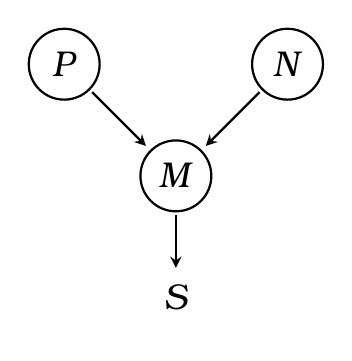
\begin{tikzpicture}[
	> = stealth, % arrow head style
	shorten > = 1pt, % don't touch arrow head to node
	auto,
	node distance = 2cm, % distance between nodes
	thick, % line style
	U/.style={circle, draw=black, inner sep=1.8pt, outer sep=1.5pt, minimum size=9mm, font=\Large},  %draw=black, fill=white
	O/.style={circle, inner sep=3.4pt, outer sep=-3pt, minimum size=9mm, font=\Large},              %draw=white, fill=white
	]
	
    % Objective items
	% Nodes and their relative positions
	\node[U] (M) {$M$};
	\node[O] (S) [below = .7 of M] {$S$};
	\node[U] (N) [above right  = 1 of M] {$N$};
	\node[U] (P) [above left = 1 of M] {$P$};
	% Paths connecting nodes
    \path[->] (P) edge (M);
	\path[->] (N) edge (M);
	\path[->] (M) edge (S);

\end{tikzpicture}
	

\end{center}\end{document}
